% !TEX root = ../Bachelorthesis.tex
%
%************************************************
% Einführung
%************************************************
\chapter{Einführung}
\label{sec:Einfuehrung}

Springer Nature ist ein weltweit führender Verlag für Forschungs-, Bildungs- und Fachliteratur mit einer breiten Palette an angesehenen und bekannten Marken. Die Verlagsgruppe bietet qualitativ hochwertige Produkte und Dienstleistungen. Springer Nature ist zudem der größte Verlag für Wissenschaftsbücher, er veröffentlicht Zeitschriften mit dem höchsten Impact in der Forschungsliteratur und gilt als Vorreiter beim Verlegen von Open-Access-Publikationen. Für Springer Nature ist es darum wichtig, auf ihren Web-Applikationen eine Suche anbieten zu können, die Suchintentionen erkennt und möglichst schnell zum gesuchten Content leitet. Die Suche wird vor allem als Hilfsmittel zur Navigation und Suche nach Literatur und Dienstleistungen genutzt. Durch die vielen von Springer Nature publizierten Zeitschriften und Querverweise in Artikeln, wird sie aber auch oft zur Suche nach Issues\footnote{Nummer der Zeitschriftenausgabe, in der sich der Artikel befindet.} und Artikeln verwendet sowie als Hilfestellung um Diagnosen zu Krankheitsbilder stellen zu können.

\section{Aufbau der Suche bei Springer Nature}
\label{sec:Einfuehrung:AufbauSucheBeiSpringerNature}

Damit die verschiedenen Verlage und Zeitschriften der Verlagsgruppe Springer Nature ihre Produkte und Dienstleistungen online anbieten können nutzt Springer Nature eine inhouse entwickelte White Label Applikation\footnote{\glqq weißes Etikett\grqq{} - eine nicht beschriftete Applikation, welche von anderen Firmen unter deren Namen verwendet werden kann}. Die White Label Applikation verwendet \textit{Apache Solr} als Suchplattform. Die Solr dient hierbei als eine der Schnittstellen zwischen dem Content-Pool von Springer und der Core-Applikation. Bei dem vom Content-Pool gelieferten Content, handelt es sich um vom Springer-Verlag publizierte Zeitschriften, Artikel, Bücher, Chapters und redaktionelle Inhalte.
\\
\\
Um das Verhalten der User auf ihren Web-Applikationen zu tracken verwendet Springer das Analysetool Webtrekk. Die daraus resultierenden Reports bieten unter anderem die Möglichkeit, \textit{Suchquery-Logs} und \textit{Click-Trough-Rates}\footnote{eine Kennzahl im Bereich Internet-Marketing um die Anzahl der Klicks auf Links im Verhältnis zu den gesamten Impressionen darzustellen} der User auszuwerten.

\begin{figure}[H]
\centering
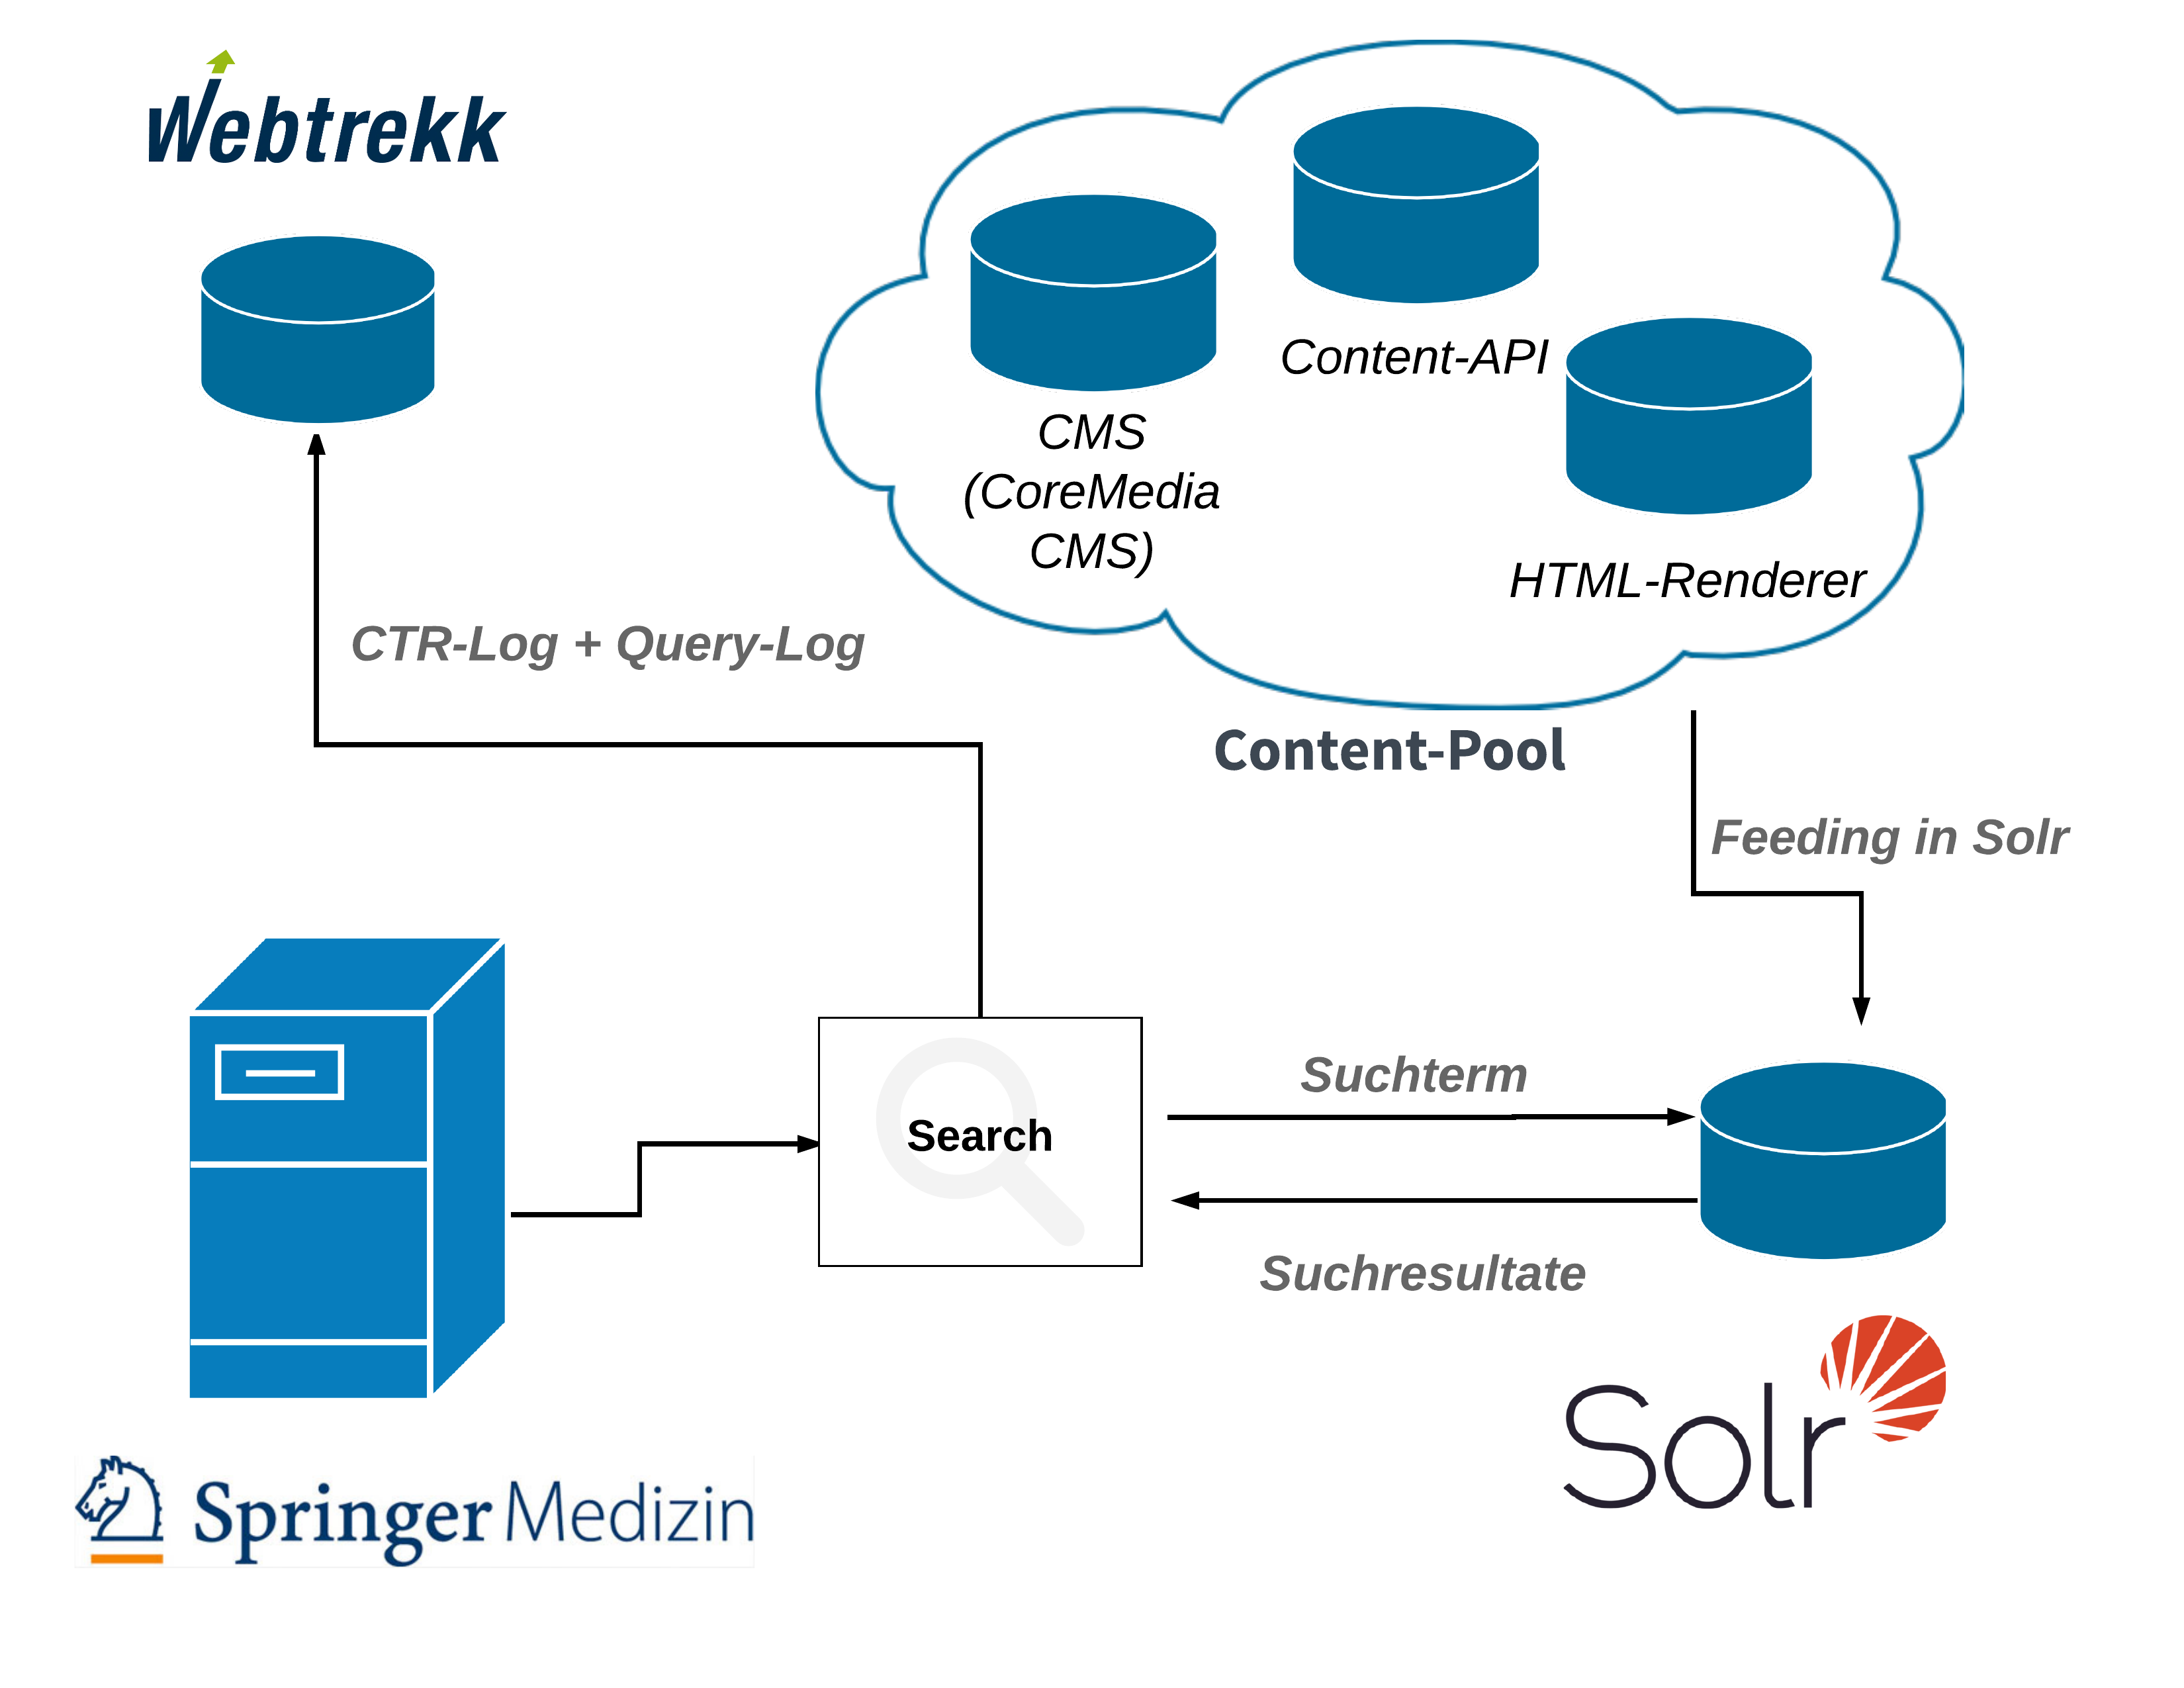
\includegraphics[width=\linewidth]{gfx/AufbauSucheSpringerNature}
\caption[Aufbau der Suche bei Springer Nature]{Aufbau der Suche bei Springer Nature}
\end{figure}

\section{Problemstellung}
\label{sec:Einfuehrung:Problemstellung}

Eine konventionelle Volltextsuche ordnet Suchergebnisse danach an, wie \textit{prominent} die Suchwörter in den einzelnen Ergebnissen vorhanden sind. Diese Art von Suche funktioniert grundsätzlich gut, solange die Prominenz der Suchwörter für die relevantesten Dokumente am höchsten ist. \cite{Bast2013}
\\
\\
Wird die Suche nun aber aus Usersicht beurteilt, fließen plötzlich ganz andere Faktoren in die Bewertung der Suchqualität ein, wie zum Beispiel: Welche Ergebnisse werden zu welchen Suchanfragen am meisten angeklickt? Oder, sind die Top-Suchergebnisse auch wirklich die für den User relevantesten Dokumente? Laut Studien kann unter Einbezug dieser User-Feedback Daten, die Sortierung der Top-Resultate in Suchmaschinen, signifikant beeinflusst werden. \cite{IWUSBI}
\\
\\
\textit{Springermedizin.de} ist ein Fortbildungs- und Informationsportal für Ärzte. Diese suchen oft mit einschlägig, fundierten Fachbegriffen nach den neuesten und relevantesten Zeitschriften, Bücher oder Publikationen. Die zeitlich aktuellsten Suchtreffer zu finden ist für Springer kein Problem. Die für den User \textit{relevantesten} jedoch schon. 

\section{Ziel der Arbeit}
\label{sec:Einfuehrung:ZielArbeit}

Durch die \textit{Click-Count-Popularität} der Suchergebnisse, können die für den User relevantesten Dokumente im Suchresultat bevorzugt werden. Die Suchmaschine würde in diesem Fall aber unabhängig der Suchanfrage immer dieselben Dokumente bevorzugen und den User in seinen Suchmöglichkeiten einschränken. Bezieht sich diese Click-Count-Popularität jedoch auf den Suchterm, sollten nur die für den Suchterm spezifisch relevanten Dokumente im Suchresultat bevorzugt werden.
\\
\\
Die Click-Count-Popularität als absoluten Wert für das \textit{Relevanzfeedback} zu nehmen, wäre jedoch auch falsch. Es muss davon ausgegangen werden, dass viele User der Qualität der Suchmaschine vertrauen und die Top-Suchresultate als die relevantesten Suchresultate betrachten. \cite{Joachims} Das Relevanzfeedback muss daher in Relation zu anderen Faktoren betrachtet werden um eine wirkliche Verbesserung der Suchergebnisqualität erzielen zu können. Ein interessanter Ansatz ist hierbei das \textit{position-based Model} (PBM). \cite{chuklin2015} Dieses geht davon aus, dass die Wahrscheinlichkeit, dass ein User ein Dokument wirklich genau analysiert bevor er es anklickt, davon abhängt wie \textit{schlecht} dieses Dokument im Suchresultat gerankt ist. Je \textit{schlechter} das Ranking des angeklickten Dokumentes ist, je \textit{höher} ist das Relevanzfeedback zu bewerten.
\\
\\
Wird nun mittels der oben erwähnten Click-Count-Popularität in Verbindung mit dem position-based Model, die Relevanz der angeklickten Dokumente berechnet, müsste davon ausgegangen werden eine Verbessung der Suchergebnisqualität erzielen zu können. Ziel dieser Arbeit ist es darum die Verbesserung der Suchqualität mittels Einbezug dieser Relevanzberechnung zu messen. Wichtig ist hierbei auch kritisch zu hinterfragen wie gut und unter welchen Vorausetzungen diese Lösung produktiv eingesetzt werden kann.  

\section{Methodik}
\label{sec:Einfuehrung:Methodik}

In der aufgestellten These werden \textit{Feedback-Strategien} für die Click-Daten Auswertung wie in \cite{Joachims} beschrieben, nicht verwendet. Diese werden in der Thesis auch nicht beachtet. Ebenfalls wird von komplexen Lern-Algorithmen wie in \cite{IWUSBI} vorgestellt, abgesehen. 
\\
\\
Die Relevanzberechnung für die angeklickten Dokumente soll auf Basis des angesprochenen \textit{position-based Model} \cite{chuklin2015} umgesetzt werden und zur Berechnung die Webtrekk-Daten verwenden. Die dabei ermittelten Scores sollen mithilfe der Boost-Funktion die angeklickten Dokumente in der Solr-Suche höher gewichten. Um vereinheitlichte Gewichtungen in der Solr-Relevanzberechnung zu wahren, müssen die Scores basierend auf den vorhanden Boost-Werten für die anderen Suchfelder des Indexes normalisiert werden.
\\
\\
Für die Bachelorthesis wird ein vorgefertigter Tracking-Report verwendet. Dieser Report wird vom \textit{Springermedizin.de}-Business über einen vordefinierten Zeitraum (beispielsweise die letzten 2 Monate) erstellt und täglich durch Webtrekk automatisch aktualisiert. Über die Webtrekk-API kann dieser Report zur Laufzeit gelesen und verarbeitet werden. Der Report enthält zu den \textit{Top-Suchqueries} auf Springermedizin.de alle angeklickten Dokumente und die wichtigsten Tracking-Informationen, wie die Anzahl der zurückgegebenen Resultate und die Position des angeklickten Dokumentes im Suchergebnis.
\\
\\
Um die aufgestellte These überprüfen zu können, muss eine passende Testumgebung aufgebaut werden. Da sich die zu verwendenden Webtrekk-Daten auf die Live-Umgebung von \textit{Springermedizin.de} beziehen, wird ein Abbild der aktuell laufenden Core-Applikation der Live-Umgebung von Springermedizin.de erzeugt und die Suche gegen die Live-Instanz der Solr ausgeführt.
\\
\\
Ist eine Testumgebung aufgebaut, muss die Verarbeitung des Webtrekk-Reports und die Relevanzberechnung in die \textit{Search-Engine} der Core-Applikation, eingebaut werden. Die Search-Engine wird über die Suche der Core-Applikation angesprochen und ist zuständig für den Aufbau der Suchanfrage für die Solr.
\\
\\
Das große Kernproblem der Überprüfung wird das Messen der Qualität der erzielten Suchergebnisse sein. Ein möglicher Ansatz hierzu könnte das Vergleichsmodell aus dem Paper \cite{Hoppe2015} sein. Dieses vergleicht eine \glqq Referenzsuchmaschine\grqq{}, mit der neu implementierten Lösung und beurteilt die Ergebnismengen der beiden Suchmaschinen auf Basis gleicher Suchanfragen. Ist ein relevantes Dokument besser gerankt als vorher, wurde die Qualität des Suchergebnisses verbessert.

\section{Gliederung und Aufbau}
\label{sec:Einfuehrung:GliederungAufbau}

Wann lesen wir was und warum?